\subsection{Performance of the Filter}
The position Kalman filter is also tuned and tested utilizing simulations. These are performed by applying some inputs to the simulation model of the system. The signals coming out of the model are then extracted and some noise is added to them. The noisy signals are used as the input to the position Kalman filter in order to evaluate its performance. The amount of noise added is the same as that present in the real sensors, whose variances are seen in \autoref{app:IMUVariances}.

As in the case of the attitude, the tuning is done by choosing the appropriate values for the covariance matrix of the states. 

This procedure starts by obtaining a good estimation of the acceleration, since the rest of the estimations depend on it. The result can be seen in \autoref{fig:sim_xbddot}.

\begin{figure}[H]
    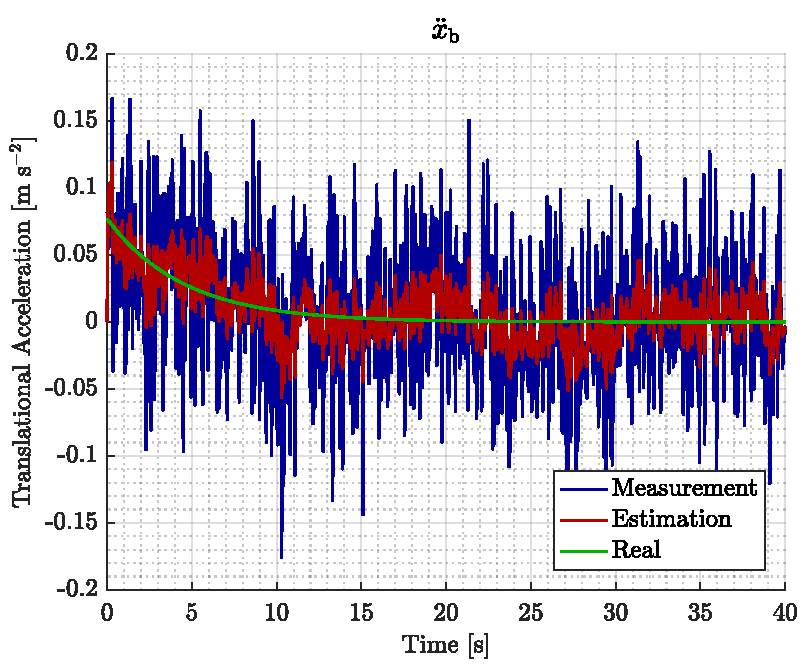
\includegraphics[width=0.5\textwidth]{figures/sim_xbddot}
    \caption{ Real value and estimation of $\ddot{x}_\mathrm{b}$}
    \label{fig:sim_xbddot}
\end{figure}
        
It is noticeable that the filter is able to reduce most of the noise that it is present on the sensor and give a good estimation of the acceleration.
 
Then, the rest of the estimations can be tuned to obtain the best result when using as well the position measurements. THe final result can be seen in \autoref{fig:sim_xbdot} and \ref{fig:sim_xn}.
\begin{figure}[H]
    \captionbox 
    {   
        Real value and estimation of $\dot{x}_\mathrm{b}$.
        \label{fig:sim_xbdot}
    }                                                                 
    {                                                                  
        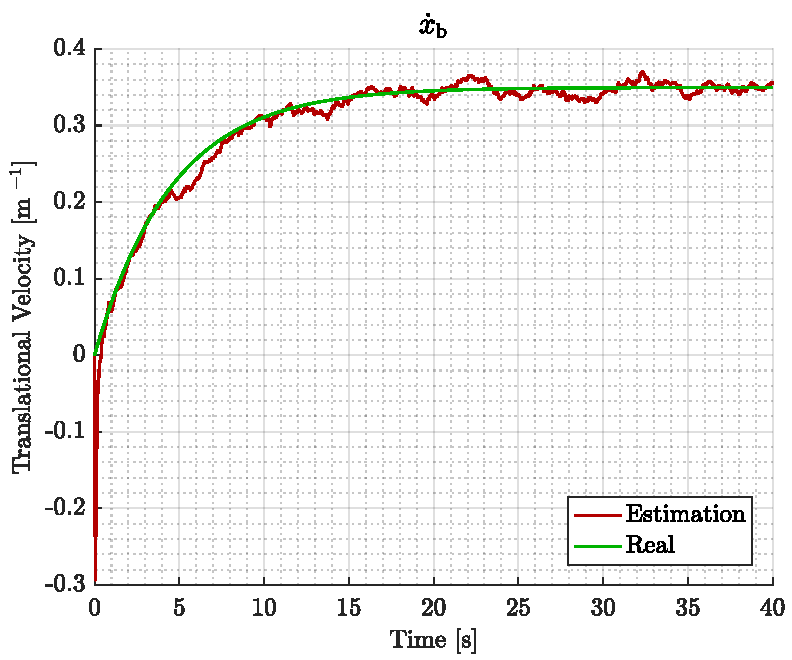
\includegraphics[width=.45\textwidth]{figures/sim_xbdot}         
    } 
    \hspace{5pt} 
    \captionbox 
    {   
        Measurement, real value and estimation of $x_\mathrm{n}$.
        \label{fig:sim_xn}
    }                                                                 
    {                                                                  
        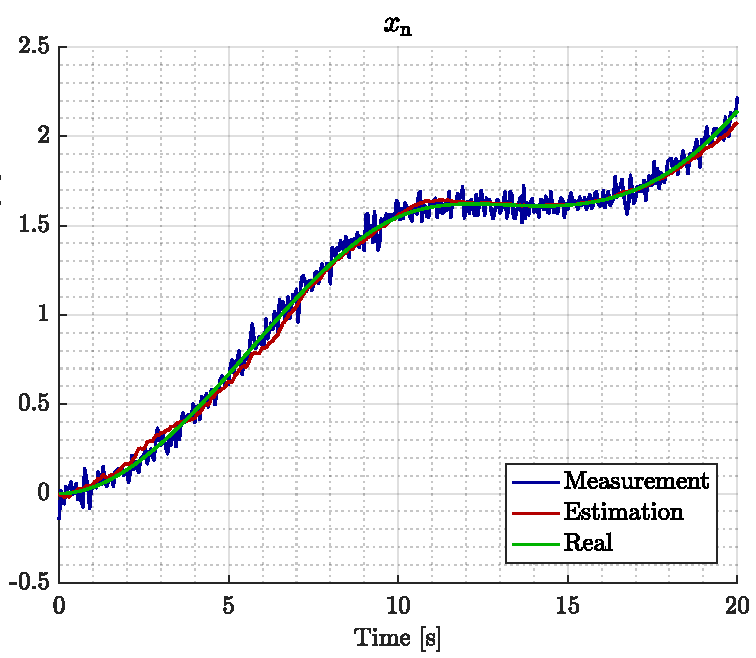
\includegraphics[width=.45\textwidth]{figures/sim_xn}         
    }                                                                   
\end{figure}        

The estimation of $\dot{x}_\mathrm{b}$ gives a good result even though there is no direct measurement of the velocity, while the estimation of $x_\mathrm{n}$ is able to remove most of the noise and be on top of the real position.
 
The final covariance matrix for the states that gives a good performance when estimation the states results as follows
%
\begin{flalign}
    \vec{Q}_\mathrm{pos} &= \mathrm{diag}\left(0,0,0,0,0,0,0,0,0 \right)\ .
\end{flalign}
